\documentclass[fleqn]{article}
\usepackage[UTF8]{ctex}
\usepackage{listings}
\usepackage{diagbox}
\usepackage[german]{babel}
\usepackage[T1]{fontenc}
\usepackage[utf8]{inputenc}
\usepackage{titlesec}
\usepackage{geometry}
\usepackage{qtree}
\usepackage{tikz}
\usepackage{ulem}
\usepackage{multirow}
\usepackage{amsmath}
\usepackage{amssymb}
\setcounter{secnumdepth}{0}
\usetikzlibrary{positioning}
\geometry{top=2.5cm, bottom=2.5cm}
\lstset{
 columns=fixed,       
 numbers=left,                                        % 在左侧显示行号
 numberstyle=\tiny\color{gray},                       % 设定行号格式
 frame=none,                                          % 不显示背景边框
 backgroundcolor=\color[RGB]{245,245,244},            % 设定背景颜色
 keywordstyle=\color[RGB]{40,40,255},                 % 设定关键字颜色
 numberstyle=\footnotesize\color{darkgray},           
 commentstyle=\it\color[RGB]{0,96,96},                % 设置代码注释的格式
 stringstyle=\rmfamily\slshape\color[RGB]{128,0,0},   % 设置字符串格式
 showstringspaces=false,                              % 不显示字符串中的空格
 language=c++,                                        % 设置语言
 breaklines,                                          % 自动换行
}

%\title{TU Chemnitz \\ Praktikum Grundlagen Technische Informatik \\ Versuch Sequ1}

%\author{Gruppe 5 - Team 5: \\ Dongze Yang \\Xiangyu Tong \\ Treshchun Kateryna}

\begin{document}

%\maketitle



\newpagestyle{main}{
    \sethead{}{}{BS 2021}
    \setfoot{}{\thepage}{}
    \headrule
    \footrule
}
\pagestyle{main}



%%%%%%%%%%%%%%%%%%%%%%%%%%%%%%%%%%%%%%%%%%%%%%%%%%
%%%%%%%     st1
%%%%%%%%%%%%%%%%%%%%%%%%%%%%%%%%%%%%%%%%%%%%%%%%%%

\section{基础概念}

\subsection{Allgemeines}

\noindent\uline{1.1 Abstraktion bedeutet...} 
 
... sich auf einen Teil der zur Verfügung stehenden Informationen zu begrenzen, 将自己限制在可用信息的一部分

... den betrachteten Gegenstand auf seine (gemäß einer Fragestellung) wesentlichen Eigenschaften zu reduzieren.
将考虑的对象减少到其(根据问题)基本属性

\noindent\uline{1.2 Die wichtigsten Grundkonzepte von Betriebssystemen sind: 最重要的基本概念}
 
Virtualisierung 虚拟化 : Das Zur-Verfügung-Stellen von Ressourcen, die tatsächlich nicht (oder nicht in der benötigten Menge/Qualität) vorhanden sind

Nebenläufigkeit 并发: Die Fähigkeit zur Ausführung von Aktivitäten außerhalb einer linearen Ordnung
 
Persistenz 稳定: Die Fähigkeit eines Zustands, die ihn erzeugende Aktivität zu überleben
 
\noindent\uline{1.3 Ob ein Betriebssystem für den Betrib folgender Systeme notwendig oder hilfreich ist?}
 
\begin{center}
    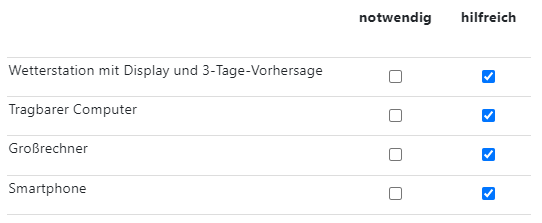
\includegraphics[scale=1]{1.png}
\end{center}

\noindent\uline{1.4 OS ist hilfreich, weil}
 
.. Aufgaben zur Interaktion von Programmen erfüllt. 完成程序交互的任务。
 
.. komplizierte, unhandliche Schnittstellen (z.B. Hardware Interfaces) vereinfacht.
简化了复杂、笨拙的接口(例如硬件接口)。

.. Programme untereinander isolieren kann.
可以将程序彼此隔离。

.. Schnittstellen vereinheitlicht. Verschiedene Netzwerkkarten können so z.B. über das gleiche Interface angesprochen werden.
接口标准化。 例如,可以通过相同的接口寻址不同的网卡。

\noindent\uline{1.5 Ein tragbarer Computer sollte über ein OS verfügen, weil:}

.. dies die Kommunikation zwischen Programmen enorm erleichtert.
这使得程序之间的通信更加容易

.. Einige Programmierer und Programmiererinnen sich nicht ausreichend um einen effizienten Stromverbrauch durch ihre Anwendungen kümmern.
一些程序员不太关心他们的应用程序的有效功耗。

.. sich sonst jede Anwendung einzeln um die Realisierung einer Netzwerkverbingdung kümmern muss.
否则每个应用程序都必须单独处理网络连接的实现。

\noindent\uline{1.6 Ein Wetterstation mit Display und 3-Tage-Vorhersage sollte über ein OS verfügen, weil}

.. es die Programmierung erleichtert. 它使编程更容易。

.. mehrere Vorgänge gleichzeitig stattfinden (z.B. Messen, Anzeigen, Vorhersagen) und diese untereinander koordiniert werden müssen.
多个过程同时发生(例如测量、显示、预测),这些过程必须相互协调。

\noindent\uline{1.7 Ein Wetterstation mit Display und 3-Tage-Vorhersage sollte NICHT über ein OS verfügen, weil}

.. sie so weniger Hauptspeicher benötigt. 所以它需要更少的主内存。

.. sie so weniger Permanentspeicher (z.B. HDD) benötigt. 因此它需要较少的永久存储(例如 HDD)。

\subsection{Standardisierung und Schnittstellen 标准化和接口}

\noindent\uline{2.1 Korrekt?}

Standardisierung ermöglicht die Portabilität von Programmcode zwischen verschiedenen Betriebssystemen.
标准化使程序代码在不同操作系统之间具有可移植性。

POSIX (Portable Operating System Interface) ist eine standardisierte Programmierschnittstelle zur Sicherstellung der Kompatibilität verschiedener Betriebssysteme.
POSIX(Portable Operating System Interface)是一种标准化的编程接口,用于保证不同操作系统的兼容性。

\noindent\uline{2.2 Zur Standardisierung von Schnittstellen eines Betriebssystem gehört zwingend:} 操作系统接口的标准化势在必行

Die semantische Spezifikation der Schnittstelle 接口的语义规范
	
Die formale Spezifikation der Schnittstelle 接口的正式规范

\noindent\uline{2.3 Textschnittstellen (Terminals) zur Benutzung von Betriebssystemen sind seit den 60er Jahren bis heute sinnvoll, weil:}  自 1960 年代以来,用于使用操作系统的文本界面(终端)一直很有用,因为
	
... für ihre Benutzung nur geringer Ressourcenbedarf besteht (wenig Bandbreite, keine GUI, ...).
使用它们只需要少量资源(带宽小,没有 GUI,...)。

... SSH, Telnet, etc. einen Standard für die Fern-Administration darstellen.
SSH、Telnet 等代表了远程管理的标准。

... im Falle von fehlerhaften Treibern ein "Notfallbetrieb" gewährleistet werden kann.
如果驱动器出现故障,可以保证“紧急操作”。

\noindent\uline{2.4 Ein Betriebssystem bietet Schnittstellen B an (z.B. für Programmierer und Anwender), mit denen Schnittstellen A (z.B. Hardware) genutzt werden können.}

\uline{Welche der folgenden Aussagen ist korrekt?}
操作系统提供接口 B(例如用于程序员和用户),可以使用接口 A(例如硬件)。 以下哪个说法是正确的?

B sollte „schöner“ sein als A.
B应该比A“更漂亮”。

Einige Möglichkeiten von A werden mittels B möglicher Weise nicht unterstützt.
B 可能不支持 A 的某些可能性。

B ist meist abstrakter als A.
B 通常比 A 更抽象。


\subsection{Designprinzipien 设计原则} 

\noindent\uline{3.1 KISS steht (im Rahmen der Vorlesung) für:} KISS 代表(在讲座的上下文中)

Keep it simple, stupid

Keep it small and simple

\noindent\uline{3.2 Wird das KISS-Prinzip eingehalten, ergeben sich folgende Vorteile:}
如果坚持 KISS 原则,则会产生以下优点

Es werden Inkonsistenzen vermieden.
避免了不一致

Die Wartbarkeit von Code wird meist verbessert. 代码的可维护性大多得到了提高。

\noindent\uline{3.3 SPOT steht (im Kontext dieser LV) für...}

Single Point of Truth

\noindent\uline{3.4 Wird das SPOT-Prinzip eingehalten, ergeben sich folgende Vorteile:}
如果坚持 SPOT 原则,则会产生以下优势:

Es werden Uneindeutigkeiten vermieden, da es nie mehrere unterschiedliche Aussagen bezüglich des gleichen Sachverhalts gibt.
避免歧义,因为对于同一问题从来没有几个不同的陈述。

\subsection{Virtuelle Maschine 虚拟机}

\noindent\uline{4.1 Vorteile. Ein Betriebssystem bietet den Anwendungen eine Repräsentation der tatsächlichen physischen Hardware an, welche in der Vorlesung als ‘virtuelle Maschine’ bezeichnet wird.}
好处。 操作系统为应用程序提供了实际物理硬件的表示,在讲座中将其称为“虚拟机”。

Tatsächliche Eigenschaften der Hardware werden vor Nutzerinnen und Nutzern "versteckt".
硬件的实际属性对用户“隐藏”。
	
Verschiedene Programme können durch Schutzmechanismen und Zugriffsrechte voreinander geschützt werden.
不同的程序可以通过保护机制和访问权限相互保护。
	
Physische Ressourcen (z.B. CPU) können unter mehreren laufenden Anwendungen aufgeteilt werden.
物理资源(例如 CPU)可以分配给多个正在运行的应用程序。

\noindent\uline{4.2 Nachteile einer virtuellen Maschine im Sinne der Vorlesung sind: 坏处}

Es wird eine zusätzliche Indirektion eingeführt, die zusätzliche Ressourcen benötigt (CPU, Speicher, ...).
引入了额外的间接寻址,它需要额外的资源(CPU、内存等)。

Man muss als Programmierer neue Konzepte verstehen.
作为程序员,您必须了解新概念。

Es ist ein zusätzlicher Aufwand für die Realisierung der virtuellen Maschine nötig.
需要额外的努力来实现虚拟机。


%%%%%%%%%%%%%%%%%%%%%%%%%%%%%%%%%%%%%%%%%%%%%%%%%%
%%%%%%%     st2
%%%%%%%%%%%%%%%%%%%%%%%%%%%%%%%%%%%%%%%%%%%%%%%%%%

\section{Microkernel, Hybridkernel, Ringarchitektur 微内核、混合内核、环形架构}

\subsection{Microkernel 微内核}

\noindent\uline{1.1	Ein Treiber sollte nicht Teil des Kernels sein weil:}
驱动程序不应该是内核的一部分,因为

Störungen durch Programmierfehler andere Treiber weitgehend ausgeschlossen werden.
可以在很大程度上排除由其他驱动程序中的编程错误引起的故障。

\noindent\uline{1.2 Es handelt sich um ein Microkernel wenn:}
它是一个微内核,如果

Nur die wichtigsten Funktionen (die nicht im Nutzermodus realisiert werden können) implementiert sind.
只实现最重要的功能(不能在用户模式下实现)。

\noindent\uline{1.3 Welche Aussagen sind richtig:}

Microkernel für PCs sind verfügbar (Mach, L4L, ...).
可以使用 PC 的微内核(Mach、L4L 等)。


\subsection{Hybridkernel 混合内核}

\noindent\uline{2.1 Welche Aussagen zu einem Hybrid-Kernel sind korrekt?}
哪些关于混合内核的陈述是正确的?

Die Qualität von Treibern mit privilegierten Modus kann mittels Kontrollen des Codes und Zertifizierung verbessert werden.
特权模式驱动程序的质量可以通过代码控制和认证来提高。

\noindent\uline{2.2 Treiber für welche Geräte können vom privilegierten Modus (im Kernel) spürbar profitieren, oder nicht profitieren?}
哪些设备的驱动程序可以或不能从特权模式(在内核中)中显着受益?

Das Dateisystem profitiert nicht, da die Festplatte zu geringe Bandbreite bietet um von den Verbesserungen spürbar zu profitieren.
文件系统没有受益,因为硬盘提供的带宽太少,无法从改进中明显受益。
	
Die Maus profitiert nicht, die Leistung ist bereits hoch genug und minimale Verbesserungen sind nicht spürbar.
鼠标没有好处,性能已经足够高,最小的改进并不明显。

\noindent\uline{2.3 Welchen Aussagen zu Treibern von sicherheitsrelevanter Hardware (z.B. Fingerabdruckssensor)  sind sinnvoll?}
哪些关于安全相关硬件(例如指纹传感器)驱动程序的陈述有意义?

Der Treiber muss aus einer überprüfbaren Quelle stammen, die Herkunft muss z.B. mit Signaturen nachgewiesen werden.
例如,驱动程序必须来自可验证的来源,来源必须用签名来证明。

Bei der Programmierung des Treibers ist besondere Sorgfalt und die Überprüfung der Software nötig.
对驱动程序进行编程时,需要特别注意和检查软件。

\noindent\uline{2.4 Wird ein Treiber (als Teil des Kerns) in den privilegierten Modus realisiert, kann die Performance gesteigert werden weil:}
如果驱动程序(作为内核的一部分)在特权模式下实现,则可以提高性能,因为:

Direkt auf andere Teile des Kerns und andere Teile zugegriffen werden kann, ohne sich an starre Interfaces zu halten.
核心的其他部分和其他部分可以直接访问,而不必坚持刚性接口。

Nicht zwischen Treiber und privilegierten Modus ungeschalten werden muss
无需在驱动程序和特权模式之间切换

\noindent\uline{2.5 Wann muss ein Betriebssystem heruntergefahren werden, wenn ein Programmierfehler auftritt?}
如果发生编程错误,操作系统何时必须关闭?

Wenn ein Treiber im privilegierten Modus einen nicht behebbaren Fehler hat (und der Treiber benötigt wird).
当处于特权模式的驱动程序出现不可恢复的错误时(并且需要该驱动程序)。

Wenn der Kernel selbst einen nicht behebbaren Fehler hat.
当内核本身有不可恢复的错误时。


\subsection{Ringarchitektur 环形架构}

\noindent\uline{3.1 Die Ring-Architektur ist ...}

... ein Hardware-Schutz, der aus Ringen mit verschiedenen Privilegien besteht.
由具有不同权限的环组成的硬件保护。

\noindent\uline{3.2 Welche Aussagen zur Intel Ring-Architektur sind korrekt?}

Im Ring 0 läuft der Betriebssystemkern.
操作系统内核在环 0 中运行。

Im Ring 3 laufen Programme.
程序在环 3 中运行。

Ring 1 und 2 werden von Windows und Linux nicht verwendet.
Windows 和 Linux 不使用环 1 和 2。

\noindent\uline{3.3 Was wird mit der Ring-Architektur geschützt?}
环结构保护什么?

Der Zugriff auf bestimmte Hardware und IO ist nur in bestimmten Ringen möglich.
只能在某些环中访问某些硬件和 IO。

Der Zugriff auf beliebige Adressen im Hauptspeicher ist nur in bestimmten Ringen möglich.
主存储器中的任何地址只能在某些环中访问。

Bestimmte Assembler/Binärbefehle können nur in bestimmten Ringen ausgeführt werden.
某些汇编/二进制指令只能在某些环中执行。


%%%%%%%%%%%%%%%%%%%%%%%%%%%%%%%%%%%%%%%%%%%%%%%%%%
%%%%%%%     st3
%%%%%%%%%%%%%%%%%%%%%%%%%%%%%%%%%%%%%%%%%%%%%%%%%%

\section{Prozess 进程}

\subsection{Prozessbegriff}

\noindent\uline{1.1	Ein Prozess ist 进程是...}

Der Code und Zustand eines Programmes. 程序的代码和状态

\noindent\uline{1.2 Welche(s) Betriebsmittel wird/werden einem Prozess in Ausführung in jedem Fall zugewiesen?}
在每种情况下,哪些资源被分配给正在执行的进程?

Prozessor 进程

Hauptspeicher 主存

\noindent\uline{1.3 Das Konzept der virtuellen Prozessoren ermöglicht es, ...}
虚拟处理器的概念使

Prozesse verzahnt auszuführen.
以相互关联的方式执行流程。(交替运行)

\subsection{Prozesskontrollblock 进程控制块}

\noindent\uline{2.1 PCB, Wozu dient der Prozesskontrollblock (PCB) 进程控制块有什么用??}
	
Zugriff auf Programminformationen. 访问程序信息。

\noindent\uline{2.2 Welche Aussage(n) ist/sind wahr für Prozesse in statischen Betriebssystemen?} 对于静态操作系统中的进程,哪些陈述是/是正确的?

Zur Laufzeit können keine neuen Prozesse erzeugt werden.
不能在运行时创建新进程。

Der Speicherort für Programmcode und Programmzustand kann sich nicht ändern während der Laufzeit.
程序代码和程序状态的存储位置在运行期间不能更改。

Der Prozesskontrollblock ist Teil des Programmzustandes.
进程控制块是程序状态的一部分。

\noindent\uline{2.3 Welche Aussage(n) ist/sind wahr für Prozesse in dynamischen Betriebssystemen?}
对于动态操作系统中的进程,哪些陈述是/是正确的?

Die Anzahl der Prozesse kann sich während der Laufzeit verändern.
进程数可以在运行时更改。

Prozesse können andere Prozesse erzeugen.
进程可以创建其他进程。

\subsection{Dispatching 调度}

\noindent\uline{3.1 Was bezeichnet man im Prozess-Kontext als Dispatching?}
什么叫做进程上下文中的调度?

Unterbrechung der Abarbeitung eines Programmes und Fortführung eines anderen Programmes
中断一个程序的处理并继续另一个程序

\noindent\uline{3.2 Welche Konsequenzen hat das Umschalten zwischen zwei Prozessen in jedem Fall?}
在每种情况下,在两个进程之间切换的后果是什么?

Änderung des Befehlszeigers
命令指针的改变

Unterbrechung der Ausführung eines Programmes durch den Prozessor
处理器执行程序的中断

\noindent\uline{3.3 Welche Aussage(n) ist/sind wahr für das Umschalten zwischen Prozessen durch Sprünge?}
对于通过跳转在进程之间进行切换,哪些陈述是/是正确的?

Ein Prozess "entscheidet" selbst, wann die Umschaltung zu einem anderen Prozess erfolgt.
一个进程自己“决定”何时切换到另一个进程。

Das Betriebssystem hat keinen Einfluss auf den Zeitpunkt der Umschaltung zwischen Prozessen.
操作系统对进程间切换的时间没有影响。

\noindent\uline{3.4 Warum ermöglicht das Merken der Fortsetzstelle bei der Umschaltung zwischen zwei Prozessesn eine größere Flexibilität?}
为什么在两个进程之间切换时记住延续点可以提供更大的灵活性?

Der laufende Prozess kann an einer "beliebigen" Stelle unterbrochen werden und die Ausführung wird später an der entsprechenden Stelle fortgesetzt.
正在运行的过程可以在“任何”点中断,然后执行将在适当的点继续。

\noindent\uline{3.5 Was bezeichnet der Begriff "Scheduling"?}
“调度”一词是什么意思?

Festlegung einer Ausführungsreihenfolge von Prozessen. 建立进程的执行顺序

\noindent\uline{3.6 Was umfasst der Mikrozustand eines Prozesses?}
过程的微观状态包括什么?

alle Informationen, die sich während der Ausführung eines Prozesses in den Registern der CPU befinden
进程执行期间 CPU 寄存器中的所有信息

\noindent\uline{3.7 Wozu dient der Kontextwechsel beim Umschalten zwischen Prozessen?}
在进程之间切换时使用的上下文更改是什么?

Fortsetzung eines Prozesses mit dem korrekten Programmzustand (Variablenbelegungen, etc.)
以正确的程序状态(变量分配等)继续流程

Fortsetzung eines Prozesses an der korrekten Stelle im Programmcode
在程序代码中的正确点继续进程

\noindent\uline{3.8 Was sind Nachteile des kooperativen Umschaltens zwischen Prozessen?}
进程间协作切换的缺点是什么?

Programmierer müssen selbstständig entscheiden an welchen Stellen im Prozess umgeschalten wird, was unter der Berücksichtigung sehr vieler Prozesse kompliziert ist.
程序员必须独立决定在进程中的哪些点进行切换,这在考虑大量进程时很复杂。

"Gierige" Prozesse könnten den Prozessor für sehr lange Zeiträume belegen und die Ausführung anderer Prozesse somit verhindern.
“贪婪”进程可能会占用处理器很长时间,从而阻止其他进程运行。

\noindent\uline{3.9 Welche Aussage(n) ist/sind wahr für das präemptive Umschalten zwischen Prozessen?}
对于进程之间的抢占式切换,哪些陈述是/是正确的?

Das Umschalten zwischen Prozessen wird von außen durch einen Wecker ausgelöst.
进程之间的切换由闹钟在外部触发。

Prozesse haben keinen direkten Einfluss auf den Zeitpunkt des Umschaltens.
进程对切换时间没有直接影响。



\subsection{Ausschluss 互斥}

\noindent\uline{4.1 Welche Aussage(n) ist/sind wahr für kritische Abschnitte?}
对于临界区,哪些陈述是/是正确的?

Kritische Abschnitte sind Codeabschnitte, die bei abwechselnder Ausführung zu Problemen führen können.
临界区是代码段,如果交替执行,可能会导致问题。

Kritische Abschnitte können nur auftreten, wenn verschiedene Programme die selben Datenstrukturen nutzen.
只有在不同的程序使用相同的数据结构时才会出现临界区。

\noindent\uline{4.2 Was muss bei der Realisierung von gegenseitigem Ausschluss berücksichtigt werden?}
实现互斥需要考虑什么?

Art der Umschaltung (kooperativ oder präemptiv)
切换类型(合作或抢占)

Anzahl der Prozessoren
处理器数量

Vorhandensein von Interrupts
存在中断

\noindent\uline{4.3 Warum ist es sinnvoll, Bedingungsvariablen für den gegenseitigen Ausschluss (Abschnittssperren) in einem atomaren Schritt zu überprüfen und zu setzen?}
为什么在一个原子步骤中检查和设置互斥(部分锁定)条件变量是有意义的?

Das Überprüfen und Setzen ist selbst ein kritischer Abschnitt. 检查和设置本身就是一个关键部分


%%%%%%%%%%%%%%%%%%%%%%%%%%%%%%%%%%%%%%%%%%%%%%%%%%
%%%%%%%     st4
%%%%%%%%%%%%%%%%%%%%%%%%%%%%%%%%%%%%%%%%%%%%%%%%%%

\section{Zustände, Prozesserzeugung, Threads}

\subsection{Zustände 状态}

\noindent\uline{1.1	Das bedingte Umschalten ermöglicht es, 条件切换使能...}

zu einem anderen Prozess zu wechseln, wenn der aktuell ausgeführte Prozess wartet (auf Betriebsmittel, etc.).
当前正在执行的进程正在等待(资源等)时切换到另一个进程。

\noindent\uline{1.2 Welche Informationen beinhaltet der Makrozustand eines Prozesses?}
进程的宏观状态包含哪些信息?

Informationen, die für die Verwaltung des Prozesses notwendig sind
管理流程所需的信息

\noindent\uline{1.3 Was sind mögliche Prozesszustandsübergänge?}
什么是可能的进程状态转换?

bereit -> laufend -> bereit

laufend -> wartend -> bereit

wartend -> bereit -> laufend

\noindent\uline{1.4 Welche Zustandswechseloperation(en) ist/sind für einen Prozess möglich, der dem Prozessor zugeordnet wurde?}
对于已分配给处理器的进程,哪些状态更改操作是可能的?

aufgeben 放弃

blockieren 锁定

\noindent\uline{1.5 Was muss im Kontext der Prozesszustände für dynamische Systeme beachtet werden?}
在动态系统的过程状态上下文中必须考虑什么?

Prozesse können existent, aber nicht aktiv sein.
进程可以存在但不处于活动状态。

Neue Prozesse können während der Laufzeit erzeugt und laufende Prozesse beendet werden.
可以在运行时创建新进程并且可以终止正在运行的进程。

\noindent\uline{1.6 Welche Zustandsänderung erfolgt für einen laufenden Prozess, wenn er durch einen höherprioren Prozess verdrängt wird?}
如果正在运行的进程被更高优先级的进程取代,它会发生什么状态变化?

laufend -> bereit

\noindent\uline{1.7 Wann tritt das Leerlaufproblem immer ein?}
什么时候总是出现怠速(空运行)问题?

Wenn alle Prozesse im Zustand "wartend" sind.
当所有进程都处于“等待”状态时。

\noindent\uline{1.8 Typische Aufgaben des Idle-Prozess sind:}
空闲进程的典型任务是:

Optimierung der Dateisysteme und Permanentspeicher (z.B. Defragmentieren).
优化文件系统和永久存储(例如碎片整理)。
	
Einschalten von Stromsparmodi.
开启省电模式。


\subsection{Prozesserzeugung 创建分支进程/线程}

\noindent\uline{2.1 Was bewirkt der fork()-Systemruf?}
fork() 系统调用有什么作用?

Es wird eine Kopie des ausführenden Prozesses erzeugt.
创建了一个正在执行的进程的副本。

\noindent\uline{2.2 Ein bereits existierender Prozess arbeitet den folgenden Code-Block ab. Wie viele zusätzliche Prozesse werden dadurch erzeugt?}
已经存在的进程执行以下代码块。 这会创建多少个额外的进程?

\begin{center}
    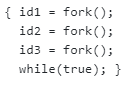
\includegraphics{2.png}
    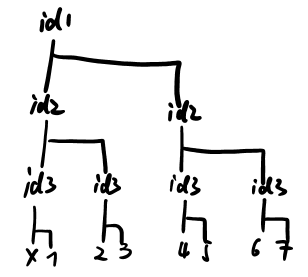
\includegraphics[scale=0.3]{3.png}
\end{center}

答案:7

\subsection{Threads}

\noindent\uline{3.1 Welche Aussage(n) ist/sind wahr für Prozesse und Threads?}
对于进程和线程,哪些陈述是/是正确的?

Ein Prozess umfasst stets mindestens einen Thread.
一个进程总是至少包含一个线程。

Ein Thread kann stets genau einem Prozess zugeordnet werden.
一个线程总是可以分配给一个进程。

\noindent\uline{3.2 Welche Informationen teilen sich die Threads eines Prozesses?}
进程的线程共享哪些信息?

Daten

Dateien
	
Programmcode

\noindent\uline{3.3 Welche Aussage(n) ist/sind wahr für User-Threads?}
对于用户线程,哪些陈述是/是正确的?

Es muss kein Kontextwechsel durchgeführt werden, wenn zwischen den Threads des gleichen Prozesses umgeschalten wird.
在同一进程的线程之间切换时无需更改上下文。

Die Blockierung eines Threads führt zur Blockierung des ganzen Prozesses.
一个线程的阻塞导致整个进程的阻塞。

Das Betriebssystem hat keinen direkten Einfluss auf das Umschalten zwischen Threads innerhalb eines Prozesses.
操作系统对进程内线程之间的切换没有直接影响。

\noindent\uline{3.4 Welche Aussage(n) ist/sind wahr für Kernel-Threads?}
对于内核线程,哪些陈述是/是正确的?

Das Umschalten kann unterschiedlich lange dauern, da unterschieden werden muss, ob zwischen Threads des gleichen Prozesses oder Threads unterschiedlicher Prozesse umgeschalten wird.
切换可能需要不同的时间长度,因为必须区分同一进程的线程之间的切换或不同进程的线程之间的切换。

Das Betriebssystem plant die Ausführung der einzelnen Threads jedes Prozesses.
操作系统调度每个进程的每个线程运行。

%%%%%%%%%%%%%%%%%%%%%%%%%%%%%%%%%%%%%%%%%%%%%%%%%%
%%%%%%%     st5
%%%%%%%%%%%%%%%%%%%%%%%%%%%%%%%%%%%%%%%%%%%%%%%%%%

\section{CPU Scheduling}

\subsection{Bedien-, Warte-, Antwortzeit}

\noindent\uline{1.1 Bedienzeit ist die Summe der Zeiten, die sich ein Prozess...}

im Running-Zustand befindet.

\noindent\uline{1.2 Wartezeit ist die Summe der Zeiten, die sich ein Prozess...}

im  Ready-Zustand oder im Blocked-Zustand befindet.

\noindent\uline{1.3 Antwortzeit ist die Summe der Zeiten, die sich ein Prozess...}

im Running-Zustand, im Ready-Zustand oder im Blocked-Zustand befindet.



\subsection{Schedules}

\noindent\uline{2.1 FIFO}

T1(0,3,2), T2(2,6,4), T3(4,4,1), T4(6,5,5), T5(8,2,3)

Anmerkung: Die Zeit zeigt immer das Ende des Intervalls der Größe 1 an; z.B. steht "1" für [0 - 1] oder "20" für [19 - 20]

\begin{center}
    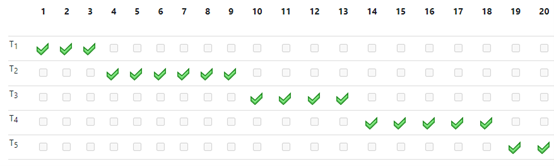
\includegraphics{4.png}
\end{center}

T1(0,3,2), T2(4,2,4), T3(6,5,1), T4(7,3,5), T5(10,6,3)

\begin{center}
    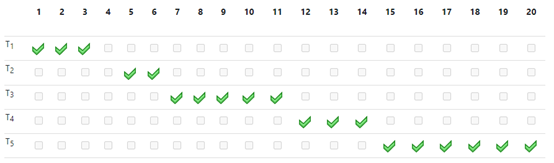
\includegraphics{5.png}
\end{center}

\noindent\uline{2.2 LCFS-PR}

T1(0,3,2), T2(2,6,4), T3(4,4,1), T4(6,5,5), T5(8,2,3)

\begin{center}
    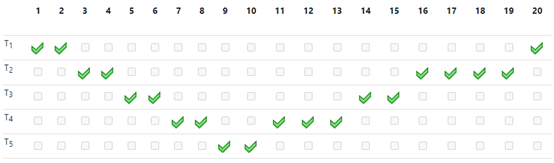
\includegraphics{6.png}
\end{center}

T1(0,7,2), T2(2,2,4), T3(5,1,1), T4(7,6,5), T5(12,4,3)

\begin{center}
    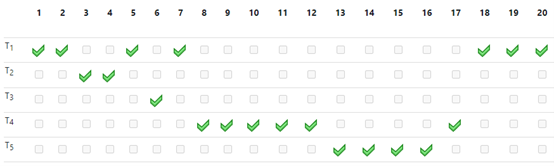
\includegraphics{7.png}
\end{center}

\noindent\uline{2.3 RR}

T1(0,3), T2(2,6), T3(4,4), T4(6,5), T5(8,2), t = 1

\begin{center}
    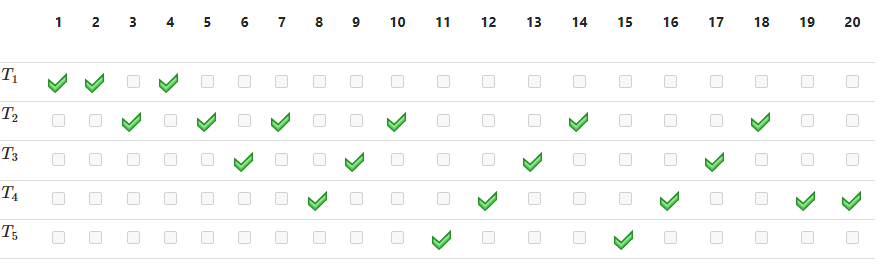
\includegraphics[scale=0.4]{21.png}
\end{center}

T1(0,2), T2(1,5), T3(3,6), T4(7,4), t = 3

\begin{center}
    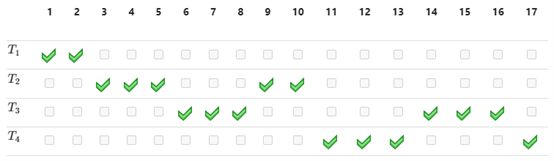
\includegraphics{8.png}
\end{center}

\noindent\uline{2.4 PRIO-NP}

T1(0,3,2), T2(2,6,4), T3(4,4,1), T4(6,5,5), T5(8,2,3)
注意:当优先级相同时,FCFS

\begin{center}
    
\includegraphics{9.png}
\end{center}

T1(0,4,5), T2(2,1,1), T3(4,2,2), T4(6,5,3), T5(6,2,4)

\begin{center}
    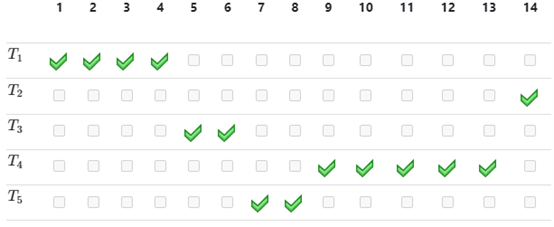
\includegraphics{10.png}
\end{center}

\noindent\uline{2.5 PRIO-P}

T1(0,3,2), T2(2,6,4), T3(4,4,1), T4(6,5,5), T5(8,2,3)

\begin{center}
    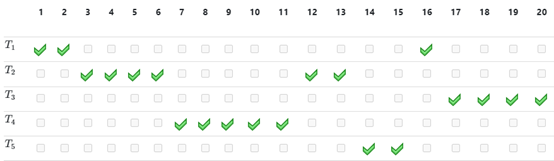
\includegraphics{11.png}
\end{center}

T1(0,4,5), T2(2,1,1), T3(3,2,6), T4(5,5,3), T5(5,2,4)

\begin{center}
    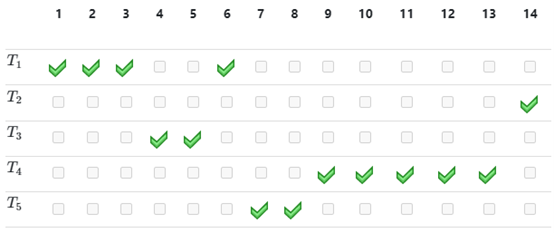
\includegraphics{12.png}
\end{center}

\noindent\uline{2.6 SJN}

T1(0,3), T2(2,6), T3(4,4), T4(6,5), T5(8,2)
注:此处为非抢占

\begin{center}
    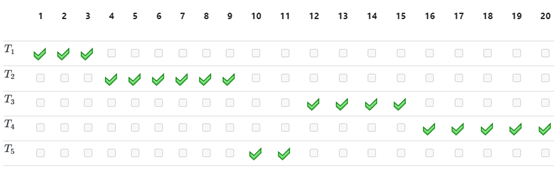
\includegraphics{13.png}
\end{center}

\noindent\uline{2.7 SRTN}

T1(0,3,2), T2(2,6,4), T3(4,4,1), T4(6,5,5), T5(8,2,3)
注:这是最短剩余相应时间的抢占版本。

\begin{center}
    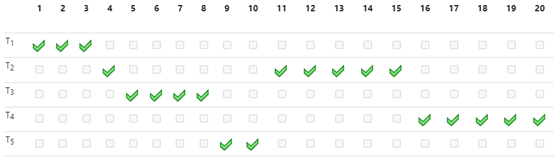
\includegraphics{14.png}
\end{center}

T1(0,7,2), T2(3,3,4), T3(4,1,1), T4(8,6,5), T5(12,3,3)

\begin{center}
    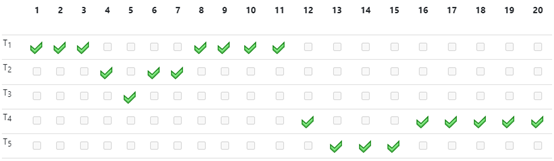
\includegraphics{15.png}
\end{center}

\noindent\uline{2.8 HRN}

T1(0,3,2), T2(2,6,4), T3(4,4,1), T4(6,5,5), T5(8,2,3)

\begin{center}
    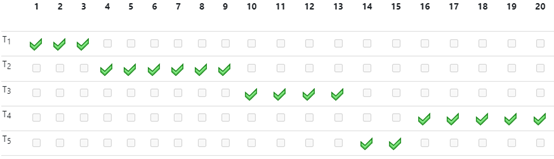
\includegraphics{16.png}
\end{center}

T1(0,7,2), T2(3,3,4), T3(4,1,1), T4(8,6,5), T5(10,3,3)
注:当出现响应率相同时,先来先服务

\begin{center}
    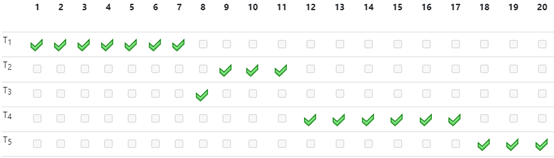
\includegraphics{17.png}
\end{center}

\noindent\uline{2.9 Multilevel Feedback}

T1(0,3), T2(2,6), T3(4,4), T4(6,5), T5(8,2)
T=1

\begin{center}
    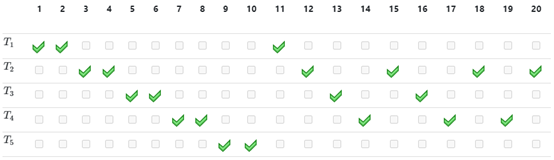
\includegraphics{18.png}
\end{center}

T1(0,3), T2(2,6), T3(4,4), T4(6,5), T5(8,2)
T = $2^{i-1}$

\begin{center}
    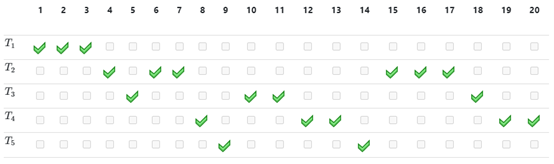
\includegraphics{19.png}
\end{center}

T1(0,4,2), T2(3,6,4), T3(4,2,1), T4(8,4,5), T5(10,4,3) 
T = $2^{i-1}$

\begin{center}
    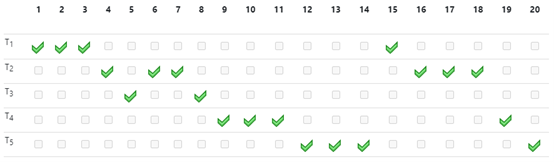
\includegraphics{20.png}
\end{center}

\subsection{RR}

\noindent\uline{3.1 RR-Antwortzeit, Ein Prozess wird - zusammen mit anderen Prozessen- mit Round Robin geplant.}
RR 响应时间,一个进程 - 与其他进程一起 - 使用循环调度。

\uline{Es sei}

b: die Bedienzeit eines Prozesses 进程的服务时间

s: die Summe der Bedienzeiten aller Prozesse in der Warteschlange 队列中所有进程的服务次数总和

n: die Anzahl der Prozesse in der Warteschlange während der Abarbeitung des Prozesses 进程正在处理时队列中的进程数

q: die Länge der Zeitscheibe 时间片的长度

(Geben Sie die Formel an! Annahme: die Bedienzeiten sind ganzzahlige Vielfache der Zeitscheibe 假设:服务次数是时间片的整数倍)

Die Anwortzeit des Prozess $t_R = b \times n$

\noindent\uline{3.2 Fairness, Round Robin gilt als fair, weil 公平,RR被认为是公平的,因为...}

bei allen Prozessen das Verhältnis von Bedienzeit zu Wartezeit etwa konstant ist.
服务时间与等待时间的比率在所有进程中大致恒定



%%%%%%%%%%%%%%%%%%%%%%%%%%%%%%%%%%%%%%%%%%%%%%%%%%
%%%%%%%     st6
%%%%%%%%%%%%%%%%%%%%%%%%%%%%%%%%%%%%%%%%%%%%%%%%%%

\section{Linearer Speicher 线性存储器}

\subsection{Verschnitt, Wahlfreier, Wiedereingliederung}

\noindent\uline{1.1	Externer Verschnitt, Welche der folgenden Speicherverwaltungsverfahren vermeidet externen Verschnitt?}
外部碎片,以下哪种仓储管理方式可以避免外部废弃物?

Ringpuffer 环形缓冲区

\noindent\uline{1.2	Wahlfreier Zugriff, Welche der folgenden Speicherverwaltungsverfahren erlauben wahlfreie Rückgabe?}
随机访问,以下哪种内存管理方法允许随机返回?

Randkennzeichnungsverfahren 边缘打标工艺
	
Halbierungsverfahren 减半过程

\noindent\uline{1.3	Automatische Wiedereingliederung, Welche der folgenden Speicherverwaltungsverfahren besitzen automatische Wiedereingliederung?}
自动重装,以下哪些存储管理方式具有自动重装功能?

Ringpuffer 环形缓冲区

Stapelverfahren 批处理

\noindent\uline{1.4	Buddy-Verfahren, Im Rahmen einer Speicherverwaltung durch Buddy-Verfahren seien B1 und B2 Buddies. B2 hat die Größe $2^k$ und die Adresse x. Geben Sie eine allgemeine Formel für die Adresse von B1 an!}
伙伴方法,在使用伙伴方法进行内存管理的上下文中,B1 和 B2 是伙伴。 B2 的大小为 $ 2^k $,地址为 x。 给出B1地址的通用公式!

x xor $2^k$



\subsection{Overhead 开销}

\noindent\uline{2.1 Ein byteadressierter Speicherbereich der Größe 1024 MiB wird in Vektordarstellung abgesetzt verwaltet. Wie groß ist der Overhead in Byte mindestens, wenn die Blockgröße 1kiB ist?}
大小为 1024 MiB 的字节寻址内存区域以矢量表示形式单独管理。 如果块大小为 1kiB,最小开销是多少?

131072

\noindent\uline{2.2 Ein byteadressierter Speicher wird mit dem Randkennzeichnungsverfahren verwaltet. Für Randtags wird jeweils ein Byte verwendet, der größte zu reservierende Bereich kann 65534 (nutzbare) Bytes, der kleinste ein (nutzbares Byte) umfassen. Dann ist im worst caseder Overhead für genutzten Speicher <\_\_\_>.}
字节寻址内存使用边缘标记方法进行管理。 1 个字节用于边缘标签,要保留的最大区域可以包含 65534 个(可用)字节,最小一个(可用字节)。 那么在最坏的情况下,使用的内存开销是<\_\_\_>。

80\%


\noindent\uline{2.3 Ordnen Sie die Algorithmen nach der erwarteten Laufzeit von kürzer nach länger!}
根据预期的运行时间从短到长对算法进行排序!

Next Fit < First Fit < Best Fit



%%%%%%%%%%%%%%%%%%%%%%%%%%%%%%%%%%%%%%%%%%%%%%%%%%
%%%%%%%     st7
%%%%%%%%%%%%%%%%%%%%%%%%%%%%%%%%%%%%%%%%%%%%%%%%%%

\section{Adressumsetzung 地址转换}

\subsection{Bindungszeit, Speicherbereiche, Fakten}

\noindent\uline{1.1	Bindungszeit, Wann findet die Adressbindung statt?}
绑定时间,地址绑定什么时候发生?

\begin{center}
    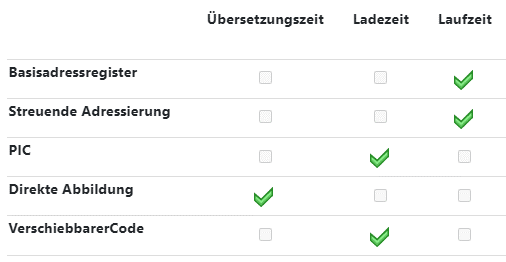
\includegraphics{22.png}
\end{center}

\noindent\uline{1.2	Speicherbereiche, Im welchen Speicherbereich werden die Datenelemente (der Programmiersprache C) typischerweise gespeichert?}
内存区域,(C 编程语言的)数据元素通常存储在哪个内存区域?

\begin{center}
    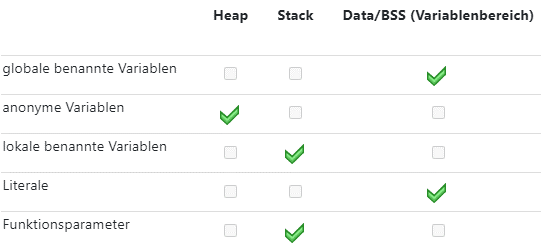
\includegraphics{23.png}
\end{center}

\noindent\uline{1.3	Fakten}

Direkte Speicherabbildung wird fast ausschließlich in monolithischen Systemen eingesetzt.
直接内存映射几乎只用于单片系统。

Beim positionsunabhängigen Code wird die Sprungweite durch Einsatz von Kettensprüngen vergrößert.
对于位置无关代码,通过使用链式跳跃来增加跳跃距离。

Der Lader platziert die Daten einer ausführbaren Datei im Speicher.
加载器将可执行文件的数据放入内存中。

Eigenrecherche: Von den Microsoft-Ausführungsformaten enthält das COM-Format keine Relokationsdaten.
内部研究:COM 格式不包含来自 Microsoft 实施例数据的任何重定位数据




\subsection{Paging 分页}

\noindent\uline{2.1 Paging}

\noindent Ein Speicher kann wahlweise mit Paging oder Segmentierug verwaltet werden. Dann gilt:
内存可以通过分页或分段进行管理。 那么以下适用:

•	Ein Eintrag in einer Seitentabelle ist kleiner als der Eintrag in einer Segementtabelle.
页表中的条目小于段表中的条目。

•	Bei Paging tritt im Vergleich zur Segmentierung ein größerer interner Verschnitt auf.
与分段相比,使用分页会产生更大的内部碎片。

•	Bei Paging kann es nicht zu einem ungültigen Offset (=> Speicherschutzverletzung) kommen.
分页期间不能发生无效偏移(=> 内存保护违规)。

\noindent\uline{2.2}

\noindent Ein System mit einer logischen Adressbreite von 32 Bit hat 4 kiB große Seiten. Speicher ist byteadressiert und wird mit Paging (einstufig) verwaltet.
逻辑地址宽度为 32 位的系统有 4 KB 页。 内存是字节寻址的,并通过分页(单级)进行管理。

Dann hat eine Seitentabelle maximal 1048576 Einträge und der Offset-Anteil in der logischen Adresse ist 12.
那么一个页表最多有 1048576 个条目,逻辑地址中的偏移部分是 12。

\noindent\uline{2.3}

\noindent Ein System mit 4 GiB zu verwaltendem Hauptspeicher besitzt eine inverse Seitentabelle. Wie wie viele Einträge hat diese, wenn die Seitengröße 16 kiB ist und der einem Prozess maximal zur Verfügung stehende Speicherbereich eines Prozesses maximal 128 kiB ist?
一个需要管理 4 GiB 主内存的系统有一个逆页表。 如果页面大小为 16 kiB 并且进程可用的最大内存区域最大为 128 kiB,那么它有多少个条目?

262144

\noindent\uline{2.4 2-stufiges Paging 二级分页}

\noindent In einem System sei die kleinste adressierbare Einheit ein Wort von 16 Bit. Eine logische Adresse umfasst 32 Bit, eine Speicherseite einen Adressraum von 216 Wörtern. Der Speicher wird mit zweistufigem Paging verwaltet. Das Seitenverzeichnis (d.h. die obere Stufe) enthält 128 Einträge.
系统中最小的可寻址单元是 16 位字。 一个逻辑地址包含 32 位,一个内存页包含 216 个字的地址空间。 内存通过两阶段分页进行管理。 页目录(即上层)包含 128 个条目。

\uline{Wie viele Einträge hat eine Seitentabelle (2. Stufe) maximal?} 页表(第二级)中的最大条目数是多少?

512

\uline{Wie viele Bit hat Eintrag in einer Seitentabelle (2. Stufe) minimal, wenn der physische Adressraum die gleiche Größe wie der logische besitzt?}
如果物理地址空间的大小与逻辑地址空间的大小相同,那么页表(第 2 级)中条目的最小位数是多少?

16



%%%%%%%%%%%%%%%%%%%%%%%%%%%%%%%%%%%%%%%%%%%%%%%%%%
%%%%%%%     st8
%%%%%%%%%%%%%%%%%%%%%%%%%%%%%%%%%%%%%%%%%%%%%%%%%%

\section{Effiziente Speicherverwaltung 高效的内存管理}

\subsection{Lokalität und Speicherhierachie 位置和存储层次结构}

\noindent\uline{1.1	Ordnen Sie die Speicherhierachie nach Zugriffsgeschwindigkeit (oben - langsam, unten - schnell)}
根据访问速度排列存储层次(上-慢,下-快)

\begin{center}
    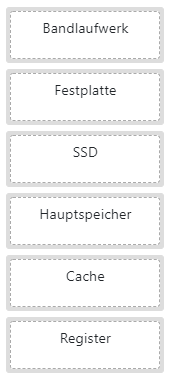
\includegraphics{24.png}
\end{center}

\noindent\uline{1.2}

\noindent Das von-Neumann-Prinzip "Ein Programm ist eine Folge von Befehlen, die in der Regel in der gegebenen Reihenfolge ausgeführt werden" unterstützt das Prinzip der ...
冯诺依曼原理“程序是通常按给定顺序执行的指令序列”支持...

Örtlichen Lokalität 当地位置

\noindent\uline{1.3}

\noindent Eine funktionale Programmiersprache (keine Schleifen, keine Variablen) unterstützt das Prinzip der ...
函数式编程语言(无循环,无变量)支持...

Örtlichen Lokalität

\noindent\uline{1.4 Eine Algorithmus, der mehrmals über ein Array iteriert, unterstützt das Prinzip der ...}
对数组进行多次迭代的算法支持...

Örtlichen Lokalität

Zeitlichen Lokalität

\noindent\uline{1.5}

\noindent Ein Speicher soll durch ein Cache beschleunigt werden, der 0,5\% der Größe des Hauptspeichers hat.
内存应该由主内存大小的 0.5\% 的缓存加速。

\noindent Ist der Cache-Zugriff ein Hit ist er 20mal schneller als ohne Cache. Jedoch wird durch die Zusätzliche Cache-Logik der Zugriff auf den Hauptspeicher im Miss-Fall um 2% langsamer als ohne Cache.
如果缓存访问成功,它比没有缓存快 20 倍。 但是,在发生故障时,附加缓存逻辑使访问主内存的速度比没有缓存时慢 2\%。

\noindent Das Verhältnis der mittleren Zugriffszeit \textbf{mit} Cache zur mittleren Zugriffzeit des gleichen Speichersystems \textbf{ohne} Cache ist
平均访问时间\textbf{mit} cache与同一存储系统\textbf{ohne} cache的平均访问时间之比为:

\uline{\textbf{1.01515}}, wenn jeder Zugriff auf eine Speicherstelle gleichwahrscheinlich ist. 如果每次访问内存位置的可能性都相等
 	
\uline{\textbf{0.535}}, wenn jeder Zugriff mit 50\%iger Wahrscheinlichkeit ein Hit ist. 如果每次访问都是以 50\% 的概率命中。

\noindent\uline{1.6}

Ein Zugriff auf eine höhere Ebene der Speicherhierachie als die Adressierte ist \uline{\textbf{Caching}}, auf eine tiefere Ebene ist \uline{\textbf{Virtualisierung}}.
访问比收件人更高级别的存储层次结构是\uline{\textbf{Caching}},更低级别是\uline{\textbf{virtualization}}。

Caching dient zur \uline{\textbf{Beschleunigung des Zugriffs}}, Virtualisierung dagegen zur \uline{\textbf{Vergrößerung des Speicherraums}}.
缓存用于\uline{\textbf{访问加速}},而虚拟化用于\uline{\textbf{增加存储空间}}。

Durch Caching und Virtualisierung können Annahmen über \uline{\textbf{die Speicherpersistenz}} gebrochen werden, was u.a. ein \uline{\textbf{Sicherheits}}-Risiko birgt.
缓存和虚拟化可以打破关于\uline{\textbf{内存持久性}} 的假设,其中包含 \uline{\textbf{安全}} 风险。


\subsection{Virtualisierung 虚拟化}

\noindent\uline{2.1 Virtualisierung}

\noindent Am häufigsten wird in modernen Systemen zur Lösung des Problems der Speicherknappheit eingesetzt: 
在现代系统中最常用于解决内存不足的问题:

Demand Paging 按需分页

\noindent\uline{2.2}

Das \uline{\textbf{Präsenzbit}} gibt an, ob sich eine bestimmte Speicherseite in einem Speicherrahmen befindet. Es befindet sich \uline{\textbf{im erweiterten Eintrag in der Seitentabelle}}. Erfolgt ein Zugriff bei nichtgesetztem Bit, wird durch \uline{\textbf{die MMU}} \uline{\textbf{ein Seitenfehler}} ausgelöst.
\uline{\textbf{Präsenzbit}} 表示某个内存页是否在内存帧中。 它位于\uline{\textbf{在页表的扩展条目中}}。 如果该位未设置,则触发\uline{\textbf{die MMU}} \uline{\textbf{a page fault}}。

Nach jedem erfolgreichen schreibenden Zugriff auf eine Speicherseite ist ihr Präsenzbit auf \uline{\textbf{wahr}} und ihr Modifikationsbit auf \uline{\textbf{wahr}} 
每次成功写入内存页后,其存在位在\uline{\textbf{true}} 上,其修改位在\uline{\textbf{true}}

\noindent\uline{2.3}

Ein System unterteilt den physischen Hauptspeicher in vier Kacheln, welche zu Beginn leer sind. Es finden Zugriffe auf Seiten in der folgenden Reihenfolge statt:
系统将物理主内存划分为四块,最初是空的。 页面按以下顺序访问:

1-2-3-4-5-1-2-5-3-4-2-1-3

Ergänzen Sie für das Ersetzungverfahren LRU (Least Recently Used) die Belegung der Kacheln nach jedem Seitenzugriff. Tragen sie dafür die Seitennummern in die jeweiligen Kästchen ein. Markieren sie zusätzlich die Zeitpunkte, bei denen ein Seitenzugriffsfehler (page fault) auftritt.
对于 LRU(最近最少使用)替换方法,在每次访问页面后添加图块的分配。 为此,请在相应的框中输入页码。 还要标记发生缺页错误的时间。

Hinweise:

•	Das Einlagern in eine leere Kachel wird nicht als Seitenzugriffsfehler gewertet.
空块中的存储不计为页面访问错误。

•	Die Speicherrahmen werden bei unechten Seitenzugriffsfehler in aufsteigender Nummerierung gefüllt
内存帧在出现错误页面访问错误时按升序填充

\begin{center}
    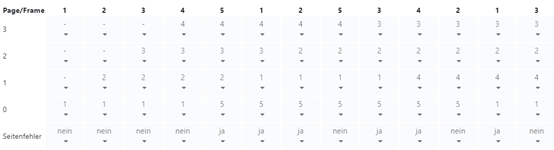
\includegraphics{25.png}
\end{center}

2.4 Konkrete Systeme 混凝土系统

\noindent BSD

•	nutze ein Algorithmus mit zwei umlaufenden Zeigern. 
使用带有两个旋转指针的算法。

•	Der Abstand der Zeiger wird angepasst entsprechend der Last. 指针之间的距离根据负载进行调整。

\noindent Windows

•	Windows nutzt eine lokale Seitenersetzungstrategie.
Windows 使用本地页面替换策略。

•	Bei Verkleinerung des Worksets erfolgt eine Auslagerung nach der LRU-Strategie.
当工作集减少时,根据 LRU 策略换出


%%%%%%%%%%%%%%%%%%%%%%%%%%%%%%%%%%%%%%%%%%%%%%%%%%
%%%%%%%     st9
%%%%%%%%%%%%%%%%%%%%%%%%%%%%%%%%%%%%%%%%%%%%%%%%%%

\section{同步问题}

\subsection{Grundformen und -abstraktionen}

\noindent\uline{1.1	Grundformen der Prozessinteraktion 进程交互的基本形式}

Datenaustausch zwischen Prozessen kommt in zwei Formen vor: Zum einen Kommunikation, bei der die Richtung des Datenaustausches wohl definiert ist, und zum anderen Kooperation., bei der dies nicht der Fall ist.

Daneben gibt es noch die Koordination, die sich um den zeitlichen Aspekt dreht.

进程之间的数据交换有两种形式:一方面是通信,其中明确定义了数据交换的方向,另一方面是协作,但情况并非如此。
还有协调,围绕时间方面。

\noindent\uline{1.2}

\begin{center}
    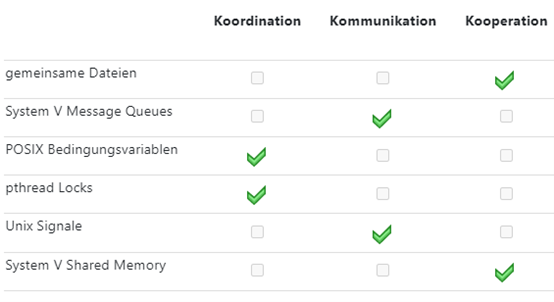
\includegraphics{26.png}
\end{center}

\noindent\uline{1.3 Welche Abstraktionen bilden die Grundlagen für}
哪些抽象构成了

•	Kommunikation:  Kanal   沟通:渠道

•	Kooperation:   Kanal   合作:渠道


\subsection{Kommunikation 沟通}

\noindent\uline{2.1 Wie ist die mögliche zeitliche Abfolge der Systemrufe bei der Kommunikation?}
通信期间系统调用的可能的时间顺序是什么?

Send - Receive

Receive – Send

\noindent\uline{2.2 Was ist ein Port?}什么是端口?

n:1 Kanal

\noindent\uline{2.3 Welche Variante(n) der Nachrichtenübergabe funktioniert unabhängig von den Zeitverhältnissen?}
无论时间条件如何,消息传输的哪个变体都有效?

Behälterübergabe, Referenzübergabe 集装箱交接、参考交接


\subsection{Kooperation 合作}

\noindent\uline{3.1 Welche Aussagen über den System V Shared-Memory-Mechanismus treffen zu?}
哪些关于 System V 共享内存机制的说法是正确的?

Geteilte Speichersegmente werden anders als der restliche Speicherraum bei Prozessbeendigung nicht freigegeben.
与其余内存不同,共享内存段在进程终止时不会被释放。

Auch der Prozess, der ein gemeinsame Speichersegment anlegt, hat keinen Zugriff darauf, bis er es einbindet (attach).
创建共享内存段的进程在附加它之前也无法访问它。

\noindent\uline{3.2 Auf welcher Adressbindungsart beruht üblicherweise shared Memory:}
哪种类型的地址绑定通常基于共享内存:
	
Streuende Abbildung 散点图



%%%%%%%%%%%%%%%%%%%%%%%%%%%%%%%%%%%%%%%%%%%%%%%%%%
%%%%%%%     st10
%%%%%%%%%%%%%%%%%%%%%%%%%%%%%%%%%%%%%%%%%%%%%%%%%%

\section{Koordination}

\noindent\uline{1.1	Wie heißen die Grundprimitiven der Koordination, auf deren Grundlagen man alle Koordinationsaufgaben lösen kann?}
协调的基本原语是什么,基于它可以解决所有协调任务?

signal und wait

\noindent\uline{1.2 Stellen Sie sicher, dass Block A stets vor Block B ausgeführt wird!}
确保块 A 总是在块 B 之前执行!

\begin{center}
    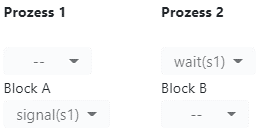
\includegraphics{27.png}
\end{center}

\noindent\uline{1.3 Stellen Sie sicher, dass Block A und Block B gleichzeitig begonnen werden können!}
确保区块A和区块B可以同时启动!

\begin{center}
    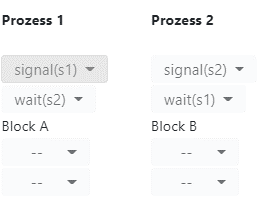
\includegraphics{28.png}
\end{center}

\noindent\uline{1.4 Stellen Sie sicher, dass Block A und Block B nie überlappend ausgeführt werden können!}
确保块 A 和块 B 永远不会重叠!

\begin{center}
    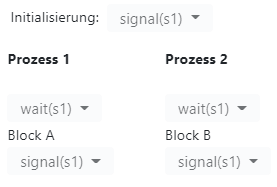
\includegraphics{29.png}
\end{center}

\noindent\uline{1.5 Stellen Sie sicher, dass Block A und Block B strickt alternierend ausgeführt werden, beginnend mit A (also A-B-A-B-...)!}
确保 A 块和 B 块交替编织,从 A 开始(即 A-B-A-B -...)!

\begin{center}
    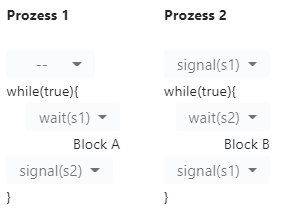
\includegraphics{30.png}
\end{center}


\noindent\uline{1.6 Welche(n) Unterschied(e) gibt es zwischen signal()/wait() und csignal()/cwait()?}

signal()/wait()和csignal()/cwait()有什么区别?

Wartet auf das Signal von csignal() niemand, verfällt es.
如果没有人等待来自 csignal() 的信号,它就会过期。

cwait() suspendiert den rufenden Prozess immer, wait() nicht.
cwait() 总是挂起调用进程,wait() 不会。




%%%%%%%%%%%%%%%%%%%%%%%%%%%%%%%%%%%%%%%%%%%%%%%%%%
%%%%%%%     st11
%%%%%%%%%%%%%%%%%%%%%%%%%%%%%%%%%%%%%%%%%%%%%%%%%%

\section{Verklemmung 死锁}

\subsection{Verklemmung}

\noindent\uline{1.1	Anzahl Prozesse und Ressourcen} 进程和资源的数量

\noindent Wieviele Prozesse und Ressourcen (kritische Abschnitte) sind mindestens nötig, um eine Verklemmung auszulösen?
至少需要多少进程和资源(临界区)才能触发死锁?

Zwei Prozesse und zwei Ressourcen. 两个进程和两个资源。

\noindent\uline{1.2 Speisenden Philosophen} 餐饮哲学家

\noindent Beim Problem der "Speisenden Philosophen" stehen die Philosophen für die \uline{\textbf{Prozesse}} und die Gabeln für die \uline{\textbf{Ressourcen}}. Eine Verklemmung entsteht in diesem Beispiel, wenn \uline{\textbf{jeder}} Philosoph genau \uline{\textbf{ein}} Gabeln gleichzeitig hält.
在“用餐哲学家”的问题中,哲学家代表\uline{\textbf{processes}},叉代表\uline{\textbf{resources}}。 在这个例子中,当 \uline{\textbf{every}} 哲学家同时持有 \uline{\textbf{one}} 个分叉时,就会出现死锁。

\noindent\uline{1.3 Coffman-Kriterien} 科夫曼标准

\noindent Welche Bedingungen zählen zu den notwendigen Coffman-Kriterien?
哪些条件是必要的科夫曼标准的一部分?

Prozesse können anderen Prozessen keine Betriebsmittel entziehen.
进程不能从其他进程中提取资源。

Ein Betriebsmittel kann nur von einem Prozess zu einem Zeitpunkt genutzt werden.
一个资源一次只能被一个进程使用。

Prozesse können Betriebsmittel besitzen, während sie auf weitere Betriebsmittel warten.
进程可以在等待更多资源的同时拥有资源。

\noindent\uline{1.4 Wählen Sie die wahren Aussagen aus.}

Es tritt stets eine Verklemmung auf, wenn das hinreichende Coffman-Kriterium erfüllt ist.
当满足足够的科夫曼准则时,总是会发生死锁。

Wenn eine Verklemmung auftritt, müssen alle Coffman-Kriterien erfüllt sein.
当发生死锁时,必须满足所有 Coffman 标准。


\subsection{Vermeidung I}

\noindent\uline{2.1 Welche der genannten Vorgehensweisen verhindern Verklemmungen?}
提到的哪些过程可以防止死锁?

Prozesse müssen alle benötigten Betriebsmittel auf einmal anfordern.
进程必须立即请求所有必需的资源。

Prozsse geben alle belegten Betriebsmittel frei, wenn sie keinen Zugriff auf ein angefordertes Betriebsmittel erhalten.
如果进程无权访问请求的资源,则进程会释放所有占用的资源。

Betriebsmittel dürfen nur noch in einer festgelegten Reihenfolge angefordert werden.
只能按规定的顺序申请设备。

\noindent\uline{2.2 Nachteile von Summenbelegung} 总分配的缺点

\noindent Was sind die Nachteile wenn man das Konzept der "Summenbelegung" nutzt, um Verklemmungen vorzubeugen?
使用“总分配”的概念来防止死锁有什么缺点?

Die möglichen Folgen sind in Systemen, in denen stets neue Prozesse hinzukommen und bestehende Prozesse beendet werden, schwer abzuschätzen.
在不断添加新进程和终止现有进程的系统中,可能的后果难以评估。

Prozesse müssen auf Betriebsmittel warten, die zwar belegt sind, aber nicht genutzt werden.
进程必须等待被占用但未使用的资源。

\noindent\uline{2.3 Eigenschaften}

\noindent Welche der genannten Eigenschaften treffen auf das Verhungern, bzw. die Verklemmung von Prozessen zu?
上述哪些属性适用于饥饿或进程死锁?

\begin{center}
    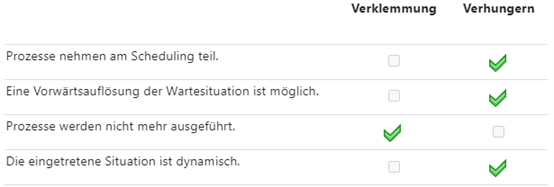
\includegraphics{31.png}
\end{center}

进程参与调度。

等待情况的前向解决是可能的。

进程不再运行。

出现的情况是动态的。


%%%%%%%%%%%%%%%%%%%%%%%%%%%%%%%%%%%%%%%%%%%%%%%%%%
%%%%%%%     st12
%%%%%%%%%%%%%%%%%%%%%%%%%%%%%%%%%%%%%%%%%%%%%%%%%%

\section{Die Entdeckung, Vermeidung und Auflösung der Verklemmung}

\subsection{Entdeckung}

\noindent\uline{1.1	Entdedckung, Der Matrix-Algorithmus ...(就是判断是否有安全状态)}

versucht eine mögliche Beendigungsreihenfolge der betrachteten Prozesse zu ermitteln, sodass keine Verklemmung entsteht.
尝试确定正在考虑的进程的可能终止顺序,以便没有死锁。

\noindent\uline{1.2 Welche Informationen benötigt der Matrix-Algorithmus über das System?}

freie Betriebsmittel
空闲资源

Zuordnung der angeforderten Betriebsmittel zu den Prozessen
将请求的资源分配给进程

Zuordnung der belegten Betriebsmittel zu den entsprechenden Prozessen
将占用的资源分配给相应的进程

\noindent\uline{1.3}

Gegeben sei ein System mit $m$ Prozessen und $n$ Betriebsmitteln.

Die aktuelle Belegung der Betriebsmittel $B$, die aktuelle angeforderten Betriebsmittel $A$,
sowie die Anzahl freien Betriebsmittel $\vec{f}$. 

Wie viele Betriebsmittel $\vec{v}$ sind insgesamt vorhanden?

$$\vec{v} = (\sum^n_{i=0} B(i,0),\sum^n_{i=0} B(i,1)\dots\sum^n_{i=0} B(i,m))+\vec{f}$$

\noindent\uline{1.4 Ein Betriebsmittelgraph ...}

beschreibt die Belegung und Anforderung aller Betriebsmittel durch Prozesse zu einem bestimmten Zeitpunkt.
描述了进程在特定时间点对所有资源的占用和需求。

\noindent\uline{1.5}

Betriebsmittelgraphen beschreiben die Belegungen und Anforderungen von Betriebsmitteln 
durch Prozesse des Systems \uline{\textbf{zu einem bestimmten Zeitpunkt}}.
 Ein Zyklus im Betriebsmittelgraph weist auf eine \uline{\textbf{bestehende}} Verklemmung hin.
 Das Anfordern eines Betriebsmittels stellt sich durch das \uline{\textbf{Einfügen}} einer Kante dar. 
 Das Belegen eines Betriebsmittels stellt sich durch das \uline{\textbf{Drehen der Richtung}} einer Kante dar. 
 Das Freigeben eines Betriebsmittels wird durch das \uline{\textbf{Entfernen}} einer Kante dargestellt

资源图描述了系统进程\uline{\textbf{在某个时间点}}对资源的分配和需求。 资源图中的循环表示\uline{\textbf{existing}} 死锁。 对资源的请求由一条边的\uline{\textbf{insert}}表示。资源的占用由一条边的\uline{\textbf{转向}}\uline{\textbf{移除}}显示的边

\noindent\uline{1.6 Eine Reduktion im Betriebsmittelgraphen ist möglich, wenn ...}

an einem Prozess nur noch eingehende Kanten vorhanden sind.
进程中只有传入边。

\noindent\uline{1.7 Die Reduktion eines Betriebsmittelgraphen ermöglicht es ...}

Anforderungskanten in Belegungskanten zu transformieren.
将需求边转换为占用边。

Belegungskanten zu entfernen.
去除覆盖边缘。


\subsection{Vermeidung II}

\noindent\uline{2.1 unsichere Situation}

Durch was zeichnet sich eine unsichere Situation bei einer aktuellen Belegungs- und Anforderungssituation aus?
什么将不安全情况与当前的占用和需求情况区分开来?

Es können nicht alle Restanforderungen eines laufenden Prozesses auf einmal erfüllt werden.
并非所有正在运行的流程的剩余要求都可以同时满足。

\noindent\uline{2.2 Wie kann verhindert werden, dass unsichere Situationen auftreten?}
我们如何防止不安全情况的发生?

Es werden nur Anforderungen gewährt, die zu einer sicheren Situation führen.
仅允许导致安全情况的要求。

\noindent\uline{2.3 Bankieralgorithmus}

Der Bankieralgorithmus wird stets bei Anforderungen in allen Situationen ausgeführt. Anforderungen werden nur gewährt, wenn die aus ihnen folgende Situation sicher ist.
在所有情况下,银行算法总是根据请求执行。 要求只有在随之而来的情况是确定的情况下才会被授予。


\subsection{Auflösung}

\noindent\uline{3.1 Was ermöglicht das Auflösen einer zyklischen Wartesituation?}
什么能够解决周期性的等待情况?

Entzug von Betriebsmitteln.
撤回资源。

Abbruch mindestens eines Prozesses.
中止至少一个进程。


%%%%%%%%%%%%%%%%%%%%%%%%%%%%%%%%%%%%%%%%%%%%%%%%%%
%%%%%%%     st13
%%%%%%%%%%%%%%%%%%%%%%%%%%%%%%%%%%%%%%%%%%%%%%%%%%

\section{Diensterbringung, Betriebsmittel, E/A-Geräte}

\subsection{Diensterbringung 服务交付/提供}

\noindent\uline{1.1	Diensterbringung 服务提供}

\noindent Worauf bezieht sich der Begriff "Driften" in der Kommunikation?
交流中的“漂流”指的是什么?

Das Vorziehen bzw. möglichst frühe Stellen von Aufträgen
尽早提出订单或下订单

Das Zurückstellen bzw. möglichst späte Entgegennehmen von Ergebnissen
尽可能推迟或接收结果

\noindent\uline{1.2 Welche der folgenden Aussagen sind zur Verbesserung des Durchsatz auf Serverseite korrekt?}
下列哪些陈述对于提高服务器端吞吐量是正确的?

Bei der Anwendung von Pipelining existieren zwischen den Teilprozessen zusätzliche Kommunikationskanäle, welche zur Entkopplung dieser Teilprozesse genutzt werden.
使用流水线时,子进程之间存在额外的通信通道,用于解耦这些子进程。

Multiplexing überträgt das Konzept von Prozesswechseln und -zuständen auf den Server: Ein "wartender" Aspekt wird zurückgestellt und ein "bereiter" Aspekt stattdessen ausgeführt.
多路复用将进程更改和状态的概念传输到服务器:“等待”方面被搁置,而“准备好”方面被执行。

Pipelining zerteilt die Aufgabe(n) des Servers in mehrere Teilschritte und -prozesse. So können neue Aufträge schon begonnen werden bevor alte Aufträge vollständig abgeschlossen sind.
流水线将服务器的任务分成几个子步骤和过程。 这意味着可以在旧作业完成之前开始新作业。

Ber Verwendung von Cloning kann es dazu kommen, dass Aufträge nicht in der Reihenfolge in der sie gestellt wurden beantwortet werden.
使用克隆可能意味着作业不会按照提交的顺序得到答复。


\subsection{Betriebsmittel}

\noindent\uline{2.1 Betriebsmittel 资源}

\noindent Warum können für First-Fit-Request und Best-Fit-Request große Anforderungen verhungern, bei FIFO jedoch nicht?
为什么大的请求对于 First-Fit-Request 和 Best-Fit-Request 会饿死,而对于 FIFO 则不行?

First-Fit- und Best-Fit-Request betrachten mehrere Anfragen, nicht nur diejenige am Ausgang der Warteschlange. Dadurch können sich Anfragen überholen.

First-Fit 和 Best-Fit 请求考虑多个请求,而不仅仅是队列出口处的请求。 因此,查询可以相互超越。

FIFO lässt kein "Überholen" von Anfragen zu - eine große Anfrage am Ausgang der Warteschlange wird also sobald wie möglich erfüllt.

FIFO 不允许请求被“超越”——队列出口处的大请求将尽快得到满足。

\noindent\uline{2.2 Welche Aufgaben hat das "Fenster", wenn die Auswahlstrategien iterativ angewandt werden?}
当迭代应用选择策略时,“窗口”有什么作用?

Durch die Verringerung der Fenstergröße beim Überspringen der ersten Anforderung kann sichergestellt werden, dass diese nicht verhungert
跳过第一个请求时减小窗口大小有助于确保它不会饿死

Es muss nicht mehr die gesamte Warteschlange betrachtet werden, damit kann Aufwand reduziert werden.
不再需要查看整个队列,可以减少工作量

\noindent\uline{2.3 Welches Ziel verfolgen die Strategien SSTF, SCAN und C-SCAN im Allgemeinen?}
SSTF、SCAN 和 C-SCAN 策略的总体目标是什么?

Sie wollen wiederholte und große Sprünge des Lesekopfes für Anfragefolgen und damit Wartezeiten vermeiden
您希望避免查询序列的读取头重复和大的跳转,从而避免等待时间


\subsection{E/A-Geräte}

\noindent\uline{3.1 E/A-Geräte}

\noindent Welche Gründe sind für die genannten Anfonderungen an Ein-/Ausgabe-Software korrekt?
对于输入/输出软件的指定要求,哪些原因是正确的?

Parallelität/Synchronität: Effiziente Treiber bremsen das System nicht aus.
并行性/同步性:高效的驱动程序不会减慢系统速度。

Fehlerbehandlung: Fehler sollen sich nicht im System ausbreiten können und so an anderen Komponenten Schaden anrichten. 
错误处理:错误不应在系统中传播,从而对其他组件造成损坏。

Parallelität/Synchronität: Einfach zu nutzende Treiber beugen Programmierfehlern vor.
并行性/同步性:易于使用的驱动程序可防止编程错误。

Abstraktion: Durch gleiche Nutzungskonzepte entsteht für den Benutzer eine einheitliche Sicht auf verschiedene Geräte
抽象:相同的使用概念为用户创建了不同设备的统一视图











































































\end{document}